% Options for packages loaded elsewhere
\PassOptionsToPackage{unicode}{hyperref}
\PassOptionsToPackage{hyphens}{url}
%
\documentclass[
]{article}
\usepackage{amsmath,amssymb}
\usepackage{lmodern}
\usepackage{iftex}
\ifPDFTeX
  \usepackage[T1]{fontenc}
  \usepackage[utf8]{inputenc}
  \usepackage{textcomp} % provide euro and other symbols
\else % if luatex or xetex
  \usepackage{unicode-math}
  \defaultfontfeatures{Scale=MatchLowercase}
  \defaultfontfeatures[\rmfamily]{Ligatures=TeX,Scale=1}
\fi
% Use upquote if available, for straight quotes in verbatim environments
\IfFileExists{upquote.sty}{\usepackage{upquote}}{}
\IfFileExists{microtype.sty}{% use microtype if available
  \usepackage[]{microtype}
  \UseMicrotypeSet[protrusion]{basicmath} % disable protrusion for tt fonts
}{}
\makeatletter
\@ifundefined{KOMAClassName}{% if non-KOMA class
  \IfFileExists{parskip.sty}{%
    \usepackage{parskip}
  }{% else
    \setlength{\parindent}{0pt}
    \setlength{\parskip}{6pt plus 2pt minus 1pt}}
}{% if KOMA class
  \KOMAoptions{parskip=half}}
\makeatother
\usepackage{xcolor}
\IfFileExists{xurl.sty}{\usepackage{xurl}}{} % add URL line breaks if available
\IfFileExists{bookmark.sty}{\usepackage{bookmark}}{\usepackage{hyperref}}
\hypersetup{
  hidelinks,
  pdfcreator={LaTeX via pandoc}}
\urlstyle{same} % disable monospaced font for URLs
\usepackage[margin=1in]{geometry}
\usepackage{graphicx}
\makeatletter
\def\maxwidth{\ifdim\Gin@nat@width>\linewidth\linewidth\else\Gin@nat@width\fi}
\def\maxheight{\ifdim\Gin@nat@height>\textheight\textheight\else\Gin@nat@height\fi}
\makeatother
% Scale images if necessary, so that they will not overflow the page
% margins by default, and it is still possible to overwrite the defaults
% using explicit options in \includegraphics[width, height, ...]{}
\setkeys{Gin}{width=\maxwidth,height=\maxheight,keepaspectratio}
% Set default figure placement to htbp
\makeatletter
\def\fps@figure{htbp}
\makeatother
\setlength{\emergencystretch}{3em} % prevent overfull lines
\providecommand{\tightlist}{%
  \setlength{\itemsep}{0pt}\setlength{\parskip}{0pt}}
\setcounter{secnumdepth}{-\maxdimen} % remove section numbering
\ifLuaTeX
  \usepackage{selnolig}  % disable illegal ligatures
\fi

\author{}
\date{\vspace{-2.5em}}

\begin{document}

\hypertarget{ssc-2022-reproducibility-workshop}{%
\subsection{SSC 2022 Reproducibility
Workshop}\label{ssc-2022-reproducibility-workshop}}

\hypertarget{join-our-slack-community}{%
\subsubsection{Join our Slack
Community}\label{join-our-slack-community}}

We are using the Statistical Education Section's Slack as a home for
this workshop, and the follow-ups afterward. You can join this Slack
\href{https://join.slack.com/t/sscstatistics-2n57302/shared_invite/zt-roolxsm8-RXc3rjbi~BMyzutPL8UJ9w}{for
free}, and we encourage you to hop on and then join the
ses2022workshop-reproducibility channel. Both Tiffany and Wesley will be
in the channel before/during/after the workshop.

\hypertarget{local-installation}{%
\subsubsection{Local Installation}\label{local-installation}}

Before the workshop, if you want to work on your own computer and your
own file system, you should complete the following steps.

\begin{enumerate}
\def\labelenumi{\arabic{enumi}.}
\tightlist
\item
  Update your version of R locally to at least 4.0, preferably
  \href{https://cran.r-project.org/}{4.2.0}.
\item
  Update your version of RStudio locally to at least 2022.02, to match
  the flow we will show.
\item
  Install Git locally
  (\href{https://git-for-windows.github.io/}{Windows};
  \href{https://www.freecodecamp.org/news/install-xcode-command-line-tools/}{Mac}).
\end{enumerate}

Regardless of whether you will work locally, or on the provided server
environment, you will need to register for a GitHub account (below).

\hypertarget{server-environment}{%
\subsubsection{Server Environment}\label{server-environment}}

An account has been created for you on Wesley's RStudio
Workbench/Server, as ses hyphen first initial + last name (e.g.,
ses-wburr). The password for all accounts has been set to the password
provided to you via the contact email. If you login to the provided URL,
you will be presented with the RStudio interface, and you can create a
new project or configure your interface as we will discuss during the
workshop.

\hypertarget{either-way}{%
\subsubsection{Either Way \ldots{}}\label{either-way}}

\begin{enumerate}
\def\labelenumi{\arabic{enumi}.}
\setcounter{enumi}{3}
\tightlist
\item
  Register for a GitHub account. This is intended as a
  \textbf{professional} account, so consider
  \href{https://happygitwithr.com/github-acct.html}{reading this guide}
  to help with account name selection and details on account types.
\end{enumerate}

\begin{figure}
\centering

\includegraphics{img/github_signup.png?raw=true}
\caption{GitHub signup}
\end{figure}

\begin{enumerate}
\def\labelenumi{\arabic{enumi}.}
\setcounter{enumi}{4}
\tightlist
\item
  Set up a SSH public/private key pair. Keys provide a more secure way
  of communicating / connecting across the internet than using
  passwords, and are \textbf{required} for GitHub use.
\end{enumerate}

Because this key creation can vary so much across different platforms,
we suggest you use RStudio's built-in utility to do it. Go to Tools
\textgreater{} Global Options\ldots\textgreater{} Git/SVN \textgreater{}
Create RSA Key.

\begin{figure}
\centering
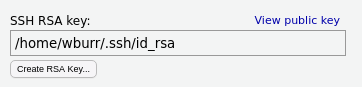
\includegraphics{img/create_RSA.png?raw=true}
\caption{RStudio Create RSA Key}
\end{figure}

RStudio prompts you for a passphrase: if you're completely new at all
this, skip the passphrase. Click ``Create'''' and RStudio will generate
an SSH key pair, stored in the files \textasciitilde/.ssh/id\_rsa and
\textasciitilde/.ssh/id\_rsa.pub. The \textasciitilde{} is a ``home''
directory, which varies by architecture, but is universal and can simply
be used.

Then, RStudio should have an option in that same screen (under Git/SVN),
to ``View Public Key''. Do that, and accept the offer to copy to your
clipboard.

Go back to GitHub, where you created your account. Click on your profile
pic in upper right corner and go to Settings \textgreater{} SSH and GPG
keys. Click ``New SSH key''. Paste your public key in the ``Key'' box.
Set a title, then click ``Add SSH key''. This will let your computer (or
account on the server) communicate seamlessly with GitHub, and will be
necessary for each account you want to use on each computer.

\hypertarget{and-now-youre-ready}{%
\subsection{And Now You're Ready}\label{and-now-youre-ready}}

You've updated RStudio and R (or are using the server), have a GitHub
account and SSH key, and you're ready for us to help you set up the
later stages.

If you want to check to see that everything is installed, try this:

\begin{enumerate}
\def\labelenumi{\arabic{enumi}.}
\tightlist
\item
  In RStudio, click File \textgreater{} New Project. Do you see an
  option to create from Version Control? If yes, good.
\item
  Select New Directory \textgreater{} Empty Project. Do you see a
  checkbox ``Create a git repository''? If yes, good, CHECK IT.
\end{enumerate}

If these aren't correct, please feel free to reach out for help!

\end{document}
